%
%
%
%%%%%%%%%%%%%%%%%%%%%%%%%%%%%%%%%%%%%%%%%%%%%%%%%%%%%%%%%%%%%%%%%%%%%%%
%                           SUBSUBSECTION                             %
%%%%%%%%%%%%%%%%%%%%%%%%%%%%%%%%%%%%%%%%%%%%%%%%%%%%%%%%%%%%%%%%%%%%%%%
%
%
%

\subsection{Спектральная плотность энергии. Формула Планка}

    К построению кривой спектральной плотности энергии $u(\omega)$ будем подходить методами статистики через количество фотонов с данной энергией в единице объема пространства.

    Фотоны подчиняются статистике Бозе-Эйнштейна, потому для среднего числа частиц с данной энергией $\varepsilon = \hbar \omega$ справедливо
    %
    \begin{equation}
        n(\varepsilon) = \frac{1}{\exp(\flatfrac{\varepsilon}{kT}) - 1} .
    \end{equation}
    %
    Спектральная плотность энергии может быть выражена как
    %
    \begin{equation}\label{eq:psd}
        u(\omega) \dd{\omega} = \hbar\omega\ n(\hbar\omega) \dd{N(\omega)} ,
    \end{equation}
    %
    где $N(\varepsilon)$~--- число мод электромагнитного поля в единице объема пространства с частотами в бесконечно малой окрестности $\omega$. Таким образом, для получения $u(\omega)$ необходимо лишь знать вид $\dv*{N}{\omega}$.

    Можно показать \cite{sivuhin_opt}, что число стоячих волн с частотами $[\omega,\omega+\dd{\omega}]$ в единице объема трехмерного пространства асимптотически ($\omega \to \infty$) распределено в соответствии с законом
    %
    \begin{equation}\label{eq:dN_of_eps_cont}
        \dd{N(\omega)} = \frac{\omega^2 \dd{\omega}}{\pi^2 v^3} .
    \end{equation}
    %
    Как и ранее, $v$ здесь обозначает скорость света в среде. При подстановке \autoref{eq:dN_of_eps_cont} в \autoref{eq:psd} спектральная плотность энергии $u(\omega)$ приобретает известный вид:
    %
    \begin{equation}
        u(\omega) = \frac{
                \flatfrac{\omega^2 \hbar\omega}{\pi^2 v^3}
        }{\exp(\flatfrac{\hbar\omega}{kT}) - 1} .
    \end{equation}
    %
    Это знаменитая формула Планка, полученная им для излучения абсолютно черного тела.

    В сферическом резонаторе спектр мод дискретен. Собственные частоты резонатора $\omega_n$ определяются нулями радиальных частей сферических мод. Известно, что радиальная часть моды зависит только от $l$ и не зависит от $m \in \qty[-l,l]$. Следовательно, $l$-я мода является $2l + 1$-вырожденной по энергии.

    Будем обозначать собственные частоты, полученные из граничных условий для $p$-поляризованной $l$-й моды, как $\omega^{lp}_n$, т.е. снабдим существующий набор $\omega_n$ дополнительными индексами. Будем также для удобства предполагать, что $\omega_n$ упорядочены по $n$: всегда выполняется $\omega_{n-1} \le \omega_n$. В таких обозначениях некоторой данной $\omega^{lp}_n$ соответствует $2l + 1$ мода с фиксированным $l$ и различными $m$. Это и есть значение функции $N(\omega)$ при $\omega = \omega^{lp}_n$ (см. далее \autoref{fig:n}\subref{fig:n_full}).

    Функции $\dv*{N}{\omega}$ же не существует вовсе. Однако можно показать, что при $\omega \to \infty$ функция $N(\omega)$ асимптотически стремится к непрерывной~--- частоты $\omega_n$ все плотнее заполняют ось частот. Рассмотрению этого случая будет посвящен отдельный раздел данной работы.

%
%
%
%%%%%%%%%%%%%%%%%%%%%%%%%%%%%%%%%%%%%%%%%%%%%%%%%%%%%%%%%%%%%%%%%%%%%%%
%                           SUBSECTION                                %
%%%%%%%%%%%%%%%%%%%%%%%%%%%%%%%%%%%%%%%%%%%%%%%%%%%%%%%%%%%%%%%%%%%%%%%
%
%
%

\subsection{Энергия излучения в сферическом резонаторе}

    В области низких частот собственные частоты резонатора располагаются относительно далеко друг от друга. Это легко заметить из \autoref{fig:n}\subref{fig:n_full}, проектируя точки функции $N(\omega)$ на ось частот: плотность заполнения оси возрастает с увеличением частоты.

    Для анализа макроскопических характеристик резонатора, как, например, плотность энергии, можно заменить дискретную последовательность $\omega_n$ непрерывной величиной $\omega$, если ошибка такого перехода не превосходит некоторой допустимой погрешности. Это выполняется при условии $kT \gg \hbar \omega_1$, т.е. когда максимум плотности энергии лежит правее минимальной собственной частоты резонатора, или, иначе, когда интегральная энергия в меньшей степени определяется модами с минимальными энергиями.

    В противном случае необходимо анализировать вклад конкретных мод в интегральное излучение. Еще раз обратимся к \autoref{eq:psd}. Проинтегрируем правую и левую части выражения по $\omega$. Представим $\dd{N}$ как $\dv*{N}{\omega}\dd{\omega}$. Получим:
    %
    \begin{equation}\label{eq:W_und}
        W \equiv \int u(\omega) \dd{\omega} =
            \int \hbar\omega\ n(\hbar\omega) \dv{N}{\omega}\dd{\omega} .
    \end{equation}
    %
    Дискретную функцию \enquote{плотности мод} $\dv*{N}{\omega}$ представим ее в виде
    %
    \begin{equation}
        \dv{N}{\omega} = \sum N(\omega_n) \delta(\omega - \omega_n) .
    \end{equation}
    %
    Тогда, очевидно, \autoref{eq:W_und} распадется на сумму вкладов отдельных мод:
    %
    \begin{equation}\label{eq:W}
        W = \sum \hbar\omega_n\ n(\hbar\omega_n) N(\omega_n)
          = \sum W_n .
    \end{equation}

    Интересно проследить, как ведут себя $W_n$ при различных температурах. При $T \to \infty$ функцию $n(\varepsilon)$ можно представить в виде
    %
    \begin{equation}
        n(\varepsilon)
            = \frac{1}{\exp(\frac{\varepsilon}{kT}) - 1}
            \approx \frac{1}{\flatfrac{\varepsilon}{kT}} = \frac{kT}{\varepsilon} ,
    \end{equation}
    %
    раскладывая экспоненту в ряд вблизи нуля. Подставляя данный результат в выражение для $W_n$, получим
    %
    \begin{equation}
        W_n = N(\omega_n) kT .
    \end{equation}
    %
    Мы приходим к классическому равномерному закону распределения энергии по степеням свободы: каждой моде\footnotemark{} соответствует энергия, равная $kT$.

    \footnotetext{
        Ранее мы вводили дополнительные индексы $l$ и $p$ в обозначения собственных частот. Очевидно, эти же индексы можно ввести и для $W_n$. Тогда смысл сказанного становится более очевиден:
        %
        \begin{equation}
            W^{lp}_n = N(\omega^{lp}_n) kT .
        \end{equation}
        %
        Значение функции $N(\omega^{lp}_n)$ определяется числом $l$ и равно $V^{-1}_\text{шара} (2l + 1)$: существует $2l + 1$ мода с одинаковым $l$, но разными $m$, соответствующих собственной частоте $\omega^{lp}_n$.
    }

    Напротив, при низких температурах $T \to 0$, можно пренебречь единицей в знаменателе $n(\varepsilon)$, получив аналог формулы Вина для отдельно взятой моды:
    %
    \begin{equation}
        W_n = \hbar\omega_n N(\omega_n) \exp(- \frac{\hbar\omega_n}{kT}) .
    \end{equation}

    Проследим, как ведут себя $W_n$ в зависимости от температуры.
    %
    \begin{enumerate}[nosep]
        \item При абсолютном нуле все моды находятся в невозбужденном состоянии: $W_n = 0$.

        \item При повышении температуры начинают возбуждаться низшие моды. При этом пока еще $W_1 > W_2$. Энергия в основном определяется первыми несколькими модами. Частотный спектр сильно дискретен~--- расстояния по частотной оси между соседними возбужденными модами здесь максимальны.

        \item Дальнейшее повышение температуры влечет \enquote{подключение} более высоких мод. Вклад в суммарную энергию все еще в большей степени определяется ранее возбужденными низшими модами. Уже отмечается $W_1 \sim W_2$.

        \item Начинают превалировать моды, возбужденные на предыдущем этапе. Максимум \enquote{плотности} энергии смещается в сторону более высоких частот.

        \item Максимум плотности энергии смещается в сторону средних и больших частот. Энергия в большей степени определяется высокими модами. Низшие моды имеют минимальный вклад в суммарную энергию. В данной области частот частотный спектр можно считать макроскопически непрерывным.
    \end{enumerate}

    Описанные эффекты изображены на \autoref{fig:plank_small_t}.
    %
    \begin{figure}[h]
        \centering
        %
        \subfloat[][]{%
            \label{fig:plank_small_t_1}%
            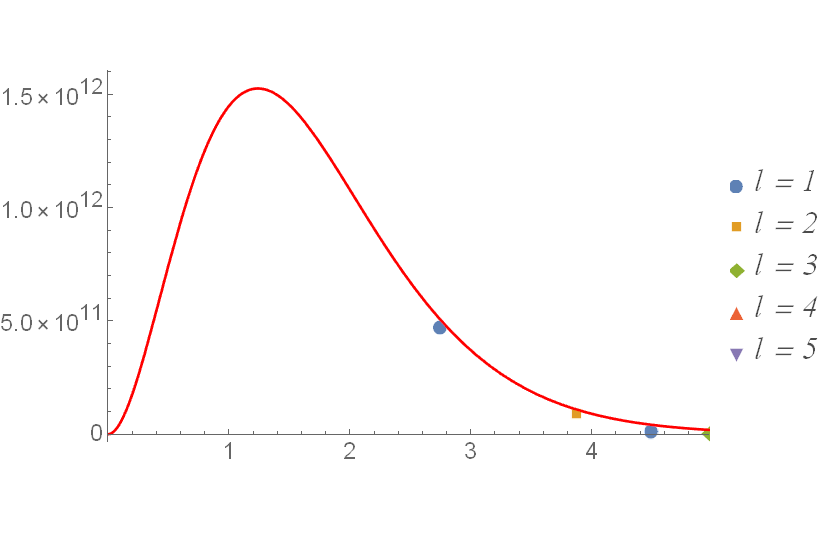
\includegraphics[width=0.45\textwidth]{plank_small_t_1}}%
        \hspace{8pt}%
        %
        \subfloat[][]{%
            \label{fig:plank_small_t_2}%
            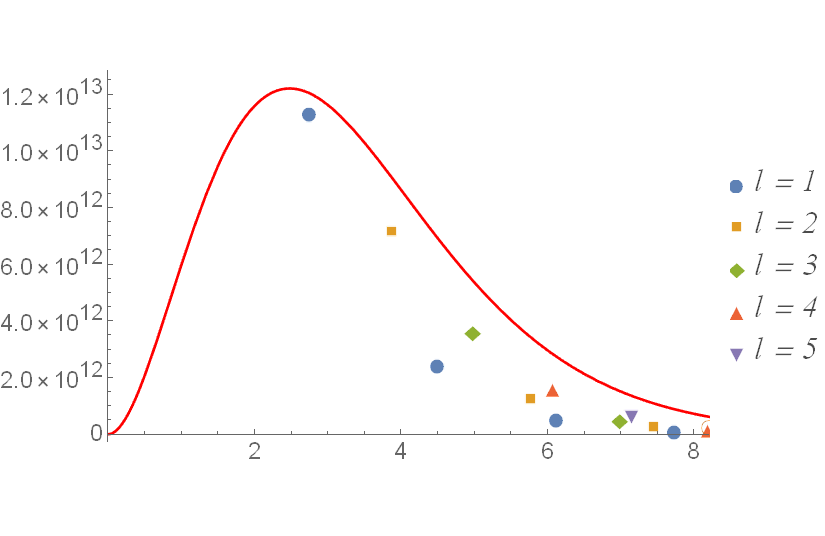
\includegraphics[width=0.45\textwidth]{plank_small_t_2}}%
        \hspace{8pt}%
        %
        \subfloat[][]{%
            \label{fig:plank_small_t_3}%
            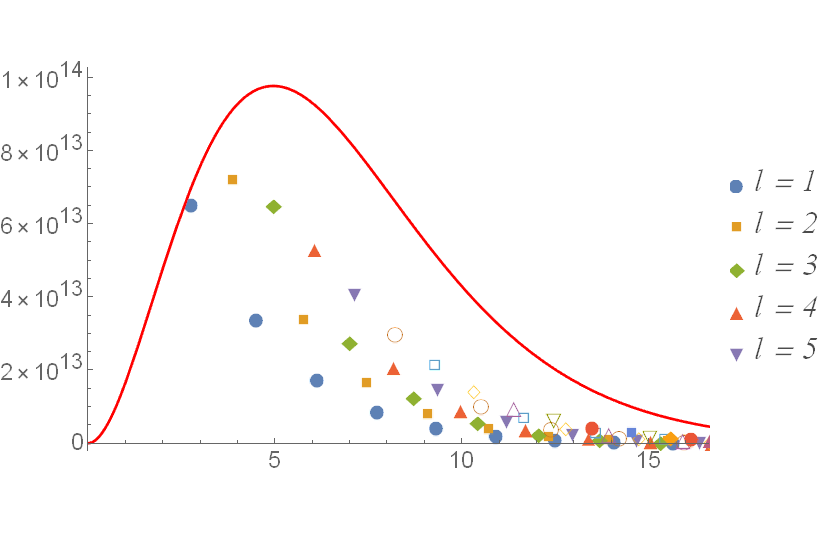
\includegraphics[width=0.45\textwidth]{plank_small_t_3}}%
        \hspace{8pt}%
        %
        \subfloat[][]{%
            \label{fig:plank_small_t_4}%
            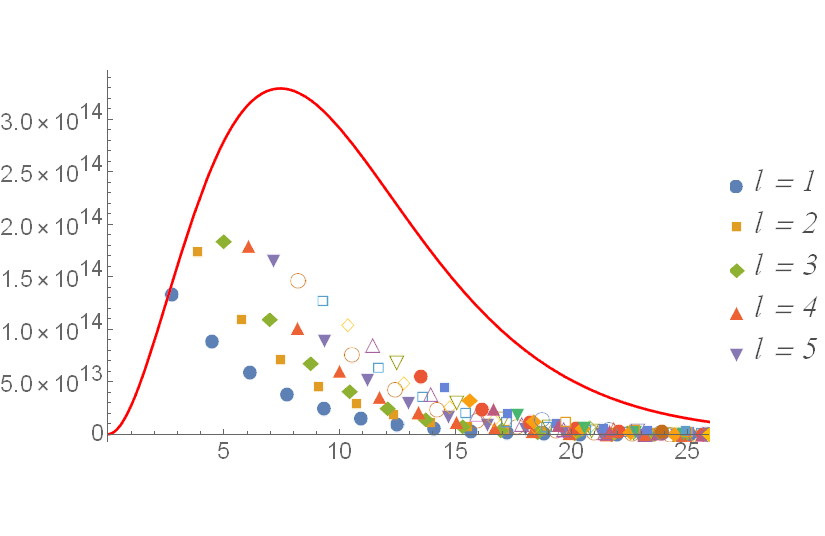
\includegraphics[width=0.45\textwidth]{plank_small_t_4}}%
        \hspace{8pt}%
        %
        \caption[]{Вклад в суммарную энергию отдельных мод вблизи нуля частот в зависимости от температуры: \subref{fig:plank_small_t_1} $T = 50K$, \subref{fig:plank_small_t_2} $T = 100K$, \subref{fig:plank_small_t_3} $T = 200K$, \subref{fig:plank_small_t_4} $T = 300K$. Размер резонатора $r_\text{шара} = 20$ микрон. Точки, соответствующие модам с одинаковым $l$, изображены одной и той же фигурой. Непрерывной линией показана кривая Планка при тех же параметрах. Числа по горизонтальной оси в единицах величины $x = \flatfrac{\omega}{v} r_\text{шара}$.} %
        \label{fig:plank_small_t}%
    \end{figure}

    Выясним соотношение температуры и размеров резонатора, при которых данные эффекты возможно наблюдать. Собственные частоты резонатора получались нами из граничных условий, которые в конечном счете сводились к уравнениям вида $f(\sqrt\lambda r_\text{шара}) = 0$ от аргумента $x = \sqrt\lambda r_\text{шара}$. Здесь $\sqrt\lambda = \flatfrac{\omega}{v}$. Отсюда $\omega = \flatfrac{v x}{r_\text{шара}}$. Величина $x$ сама по себе зависит только лишь от вида функции $f$, который вполне определен. Таким образом, собственные частоты напрямую зависят от размеров резонатора.

    Эффекты, связанные с дискретностью мод, проявляются при $kT \sim \hbar \omega_1$. Подставляя сюда представление $\omega$ через $x$, получим:
    %
    \begin{equation}
        T \sim \frac{\hbar v}{k} \frac{x_1}{r_\text{шара}} .
    \end{equation}
    %
    Численно $x_1 \approx 2.74$. Таким образом,
    %
    \begin{equation}
        T \sim \frac{6 \times 10^{-3}}{n r_\text{шара}} .
    \end{equation}
    %
    Для того, чтобы рассматриваемые эффекты проявились при комнатной температуре ($T = 300K$) в резонаторе, заполненном воздухом ($n = 1$), необходимо, чтобы радиус резонатора составлял порядка 20 микрон. Интересно, что при таких размерах $\omega_1$ будет лежать в области инфракрасного излучения. Учитывая, что оптические диэлектрические резонаторы с МШГ имеют характерные размеры порядка десятков-сотен микрон \cite{microresonators}, наблюдать рассматриваемые эффекты вполне возможно в реальных резонаторных системах.

%
%
%
%%%%%%%%%%%%%%%%%%%%%%%%%%%%%%%%%%%%%%%%%%%%%%%%%%%%%%%%%%%%%%%%%%%%%%%
%                           SUBSECTION                                %
%%%%%%%%%%%%%%%%%%%%%%%%%%%%%%%%%%%%%%%%%%%%%%%%%%%%%%%%%%%%%%%%%%%%%%%
%
%
%

\subsection{Построение кривой спектральной плотности энергии}

    Перейдем к построению кривой спектральной плотности энергии поля в резонаторе в области больших частот, где дискретность мод уже не так существенна.

    Наша задача сводится к следующему. Необходимо показать, что и в случае сферического резонатора наблюдается асимптотическое поведение $\dv*{N}{\omega} \sim \omega^2$ при больших $\omega$. Для этого необходимо посчитать $\dv*{N}{\omega} \approx \flatfrac{\Delta N}{\Delta \omega}$ по существующему спектру мод, т.е. фактически произвести свертку функции дискретного аргумента $N(\omega^{lp}_n) = 2l + 1$ с окном $\Delta \omega$.

    Изобразим функцию $N(\omega_n)$ (\autoref{fig:n}). Каждая \enquote{строчка} функции соответствует аргументам $\omega^{lp}_i$ для обеих значений $p$ и фиксированного значения $l$. Численно $\omega^{lp}_i$ являются нулями радиальных функций. С увеличением $l$ независимо от поляризации увеличивается также и положение самого левого нуля радиальной функции. Нули радиальных функций обеих поляризаций находятся близко друг к другу. Асимптотически при $i \to \infty$ расстояние между соседними нулями каждой из радиальных функций стремится к $\pi$.
    %
    \begin{figure}[h]
        \centering
        %
        \subfloat[][]{%
            \label{fig:n_all}%
            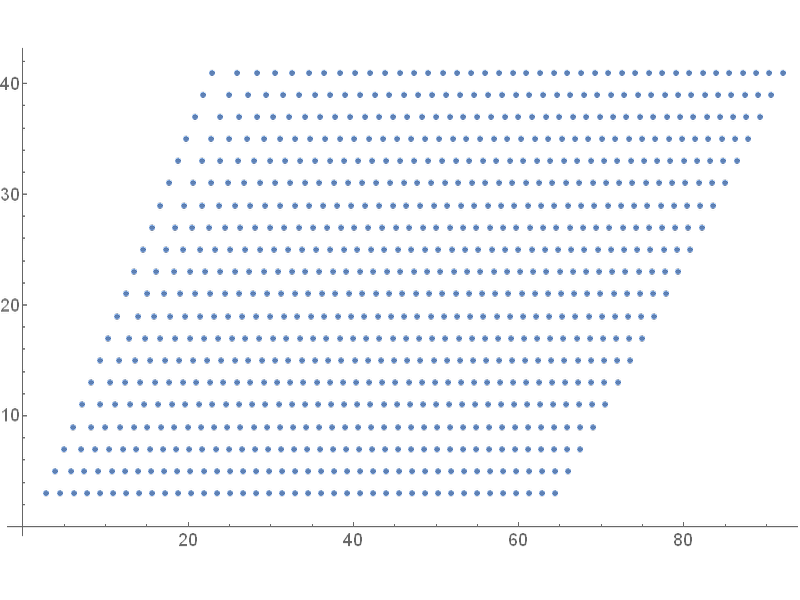
\includegraphics[width=0.45\textwidth]{n}}%
        \hspace{8pt}%
        %
        \subfloat[][]{%
            \label{fig:n_full}%
            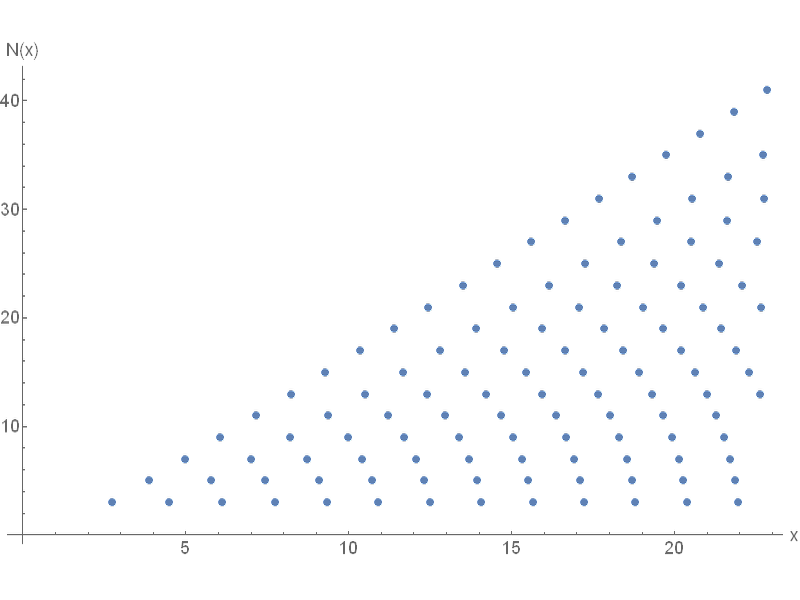
\includegraphics[width=0.45\textwidth]{n_full}}%
        \hspace{8pt}%
        %
        \caption[]{Функция $N(\omega_n)$ (аргумент в относительных единицах). Параметр $l_{max} = 300$. На \subref{fig:n_full} увеличена область $\omega < \Omega$. %
        } %
        \label{fig:n}%
    \end{figure}

    Описанная картина говорит о следующем. Пусть мы имеем некоторый рассчитанный конечный набор $\omega^{lp}_n$, $n = 1, 2, \dots, n_{max}$, полученный из $2 * (l_{max} - l_{min})$ различных базовых мод (двойка соответствует числу возможных поляризаций). В области $0 < \omega \le \Omega = \min_p{\omega^{l_{max}p}_{i_{min}}}$, где $i_{min}$~--- индекс самого левого нуля $l_{max}$-й радиальной функции $p$-й поляризации, имеется полная информация о функции $N(\omega_n)$. Иными словами, в этой области она построена по всем своим возможным аргументам. В области $\omega > \Omega$ отсечены значения функции $N(\omega^{lp}_n)$ с $l > l_{max}$, потому она не пригодна для дальнейшего рассмотрения. Под $l_{min}$ здесь понимается минимальное физически возможное значение $l$. Ранее было показано, что $l_{min} = 1$.

    На \autoref{fig:dndx} изображена функция $\flatfrac{\Delta N}{\Delta \omega}$ в области $\omega < \Omega - \Delta\omega / 2$. Видно, что результат свертки визуально похож на квадратичную функцию. Это подтверждает также и изображенная поверх множества точек непрерывная функция. Коэффициенты функции были получены методом минимизации функционала квадратичной нормы отклонения непрерывной функции от дискретных точек $\flatfrac{\Delta N}{\Delta \omega}$. По \autoref{fig:dndx}\subref{fig:dndx_mag} видно, что дискретные точки ложатся на непрерывную кривую уже при совсем небольших значениях $\omega_n$. Следует, однако, понимать, что реальный спектр излучения является дискретным, поэтому использовать функцию $\flatfrac{\Delta N}{\Delta \omega}$ для анализа излучения при малых значениях $\omega$ и малых температурах не совсем корректно (см. ниже).
    %
    \begin{figure}[h]
        \centering
        %
        \subfloat[][]{%
            \label{fig:dndx_all}%
            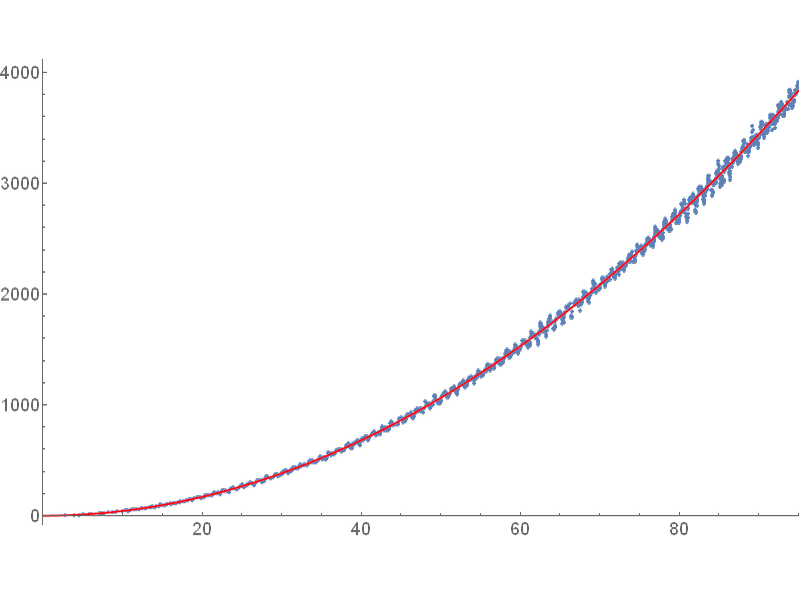
\includegraphics[width=0.45\textwidth]{dndx}}%
        \hspace{8pt}%
        %
        \subfloat[][]{%
            \label{fig:dndx_mag}%
            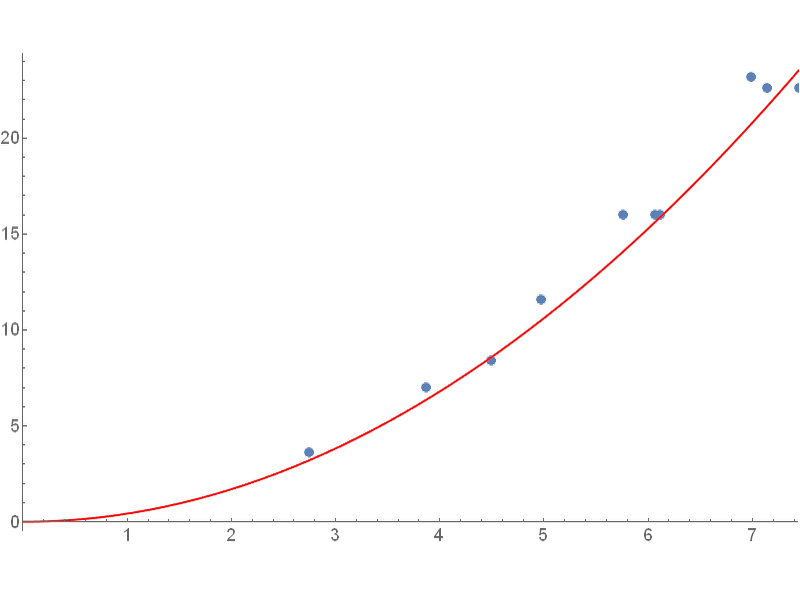
\includegraphics[width=0.45\textwidth]{dndx_mag}}%
        \hspace{8pt}%
        %
        \caption[]{Функция $\flatfrac{\Delta N}{\Delta \omega}$ (аргумент в относительных единицах), дискретная и непрерывная. Параметр $l_{max} = 100$. Размер окна~--- 5 относительных единиц. На \subref{fig:dndx_mag} увеличена область вблизи нуля. %
        } %
        \label{fig:dndx}%
    \end{figure}

    Более детально вопрос непосредственного получения $\flatfrac{\Delta N}{\Delta \omega}$ описан в \autoref{sec:getting_plank_formula}.

    Итак, мы показали, что асимптотически $\flatfrac{\Delta N}{\Delta \omega} \sim \omega^2$, причем данное соответствие имеет место уже при совсем небольших значениях $\omega$. Это, в свою очередь, доказывает справедливость формулы Планка и в случае сферических резонаторов. На \autoref{fig:plank} изображена кривая спектральной плотности энергии по дискретным данным с наложенной на нее классической непрерывной кривой. Как и ожидалось, кривые совпадают.
    %
    \begin{figure}[h]
        \centering
        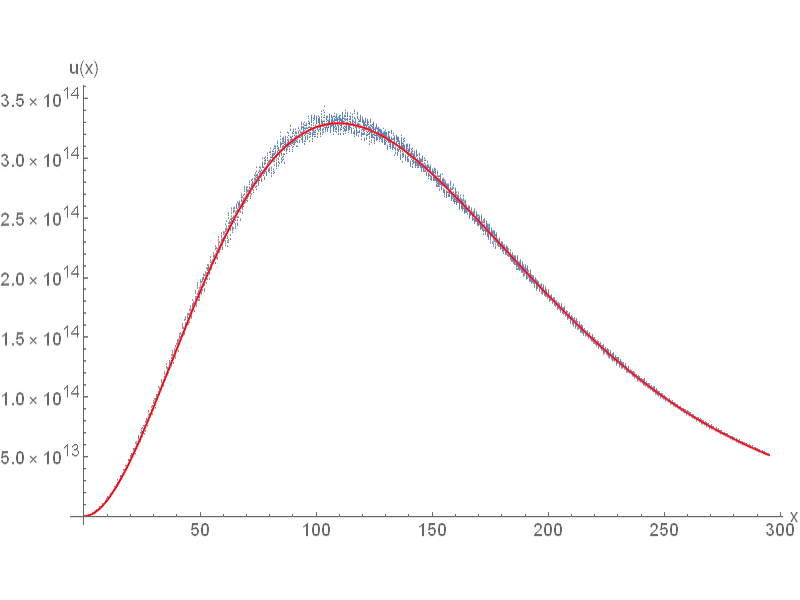
\includegraphics[width=0.5\textwidth]{plank}
        \caption[]{Планковская кривая, практическая (дискретная, построенная на данных \autoref{fig:dndx}; параметр $l_{max}$ увеличен до $300$) и теоретическая (непрерывная). Единицы относительные.}
        \label{fig:plank}
    \end{figure}
